\section{Bugs}
\doom{} is known for its stability partly thanks to a development process using seven compilers and systems. Nonetheless it shipped with a few bugs.








\subsection{Flawed collision detection}
There is rare collision detection bug which was first brought to light (and subsequently explained in depth) by Colin "cph" Phipps in his article "Shooting Through Things".\\
\par
\fq{A monster is getting too close for comfort. You shoot at it, and miss. If you are unlucky, the monster kills you. But you were so sure that you were pointing right into the monster, that so close as you were you couldn't have missed. Perhaps it was the chaingun playing up, shooting all the bullets off to one side. Perhaps the game was written by a bunch of losers who failed their high-school geometry. Or perhaps, in the heat of the moment, you really did miss; nobody's perfect.\\
\par
Well I have good news. You can blame your tools.}{Colin Phipps}\\
\par
Some enemies can be really big, almost ten times bigger than the player (16 units) like in the case of the Spider Mastermind (128 units). As we saw on page \pageref{E1M1_blockmap}, \doom{} uses blockmaps to speed up intersection with walls and things. If a Thing is on the edge of block and the player is a bit unlucky a miss can be calculated when it should have been a hit.

\fullimage{beasts_sizes.png}
\vspace{-1cm}
\fullimage{beasts_sizes2.png}


\rawdrawing{collision_miss}
\par
It is possible to miss a SpiderDemon in a hallway. In the single room map above, the green player on the left is firing at a red enemy 128 units wide on the right (probably a SpiderDemon). The blue grid shows the blockmap's alignment.\\
\par
 The line of the bullet and the radius of the monster clearly overlap. This should be a hit. But only content of blockmaps \cw{0}, \cw{1}, and \cw{2} will be checked resulting in test with walls \cw{D}, \cw{A}, and \cw{B}. Since the enemy is in block \cw{5} and the bullet doesn't cross it, the hit is not registered.\\
 \par
 This issue is not reserved to very large monsters. It can happen with any enemies depending on how close they are to the player and the blockmaps alignment.







\subsection{Slime trail}
A slime trail happens when there is an horizontal screen space gap between two walls. Visplanes "leaks" between the space, resulting in graphic glitches. This was a known issue during development that due to deadline and rarity of the occurrence was never fixed. John Carmack mentioned it when \cw{doombsp} source code was released.\\
\par
\fq{There IS a bug in here that can cause up to a four pixel wide column to be drawn out of order, causing a more distant floor and ceiling plane to stream farther forward than it should.  You can sometimes see this on E1M1 looking towards the imp up on the ledge at the entrance to the zig zag room.  A few pixel wide column of slime streams down to the right of the walkway.  It takes a bit of fidgeting with the mouse to find the spot.  If someone out there tracks it down, let me know...
}{John Carmack}\\
\par


\fullimage{slime_trail.png}

The issue can actually be far wider than four pixels if one knows where to look.\\
\par
\fullimage{big_slime_trail.png}
\par
This particular instance of slime trail has to do with the way maps were preprocessed via \cw{doombsp}. As it was explained on page \pageref{Binary Space Partitioning: Theory}, the technique looked like "sunshine and rainbows" but when applied to a system with finite precision, subtle issues arose.\\
\par
 Once again, let's take an example. The two previous screenshots where taken in the very first map the player encountered, E1M1 in a zigzag section surrounded by toxic green liquid. At first glance, there is nothing unusual here but when taking a look at how it was sliced during binary partitioning, an interesting special case appears.\\
\par
Line \cw{A} was selected as a splitter. As it crosses lines \cw{B} and \cw{G}, two segments are created as \cw{B1}, \cw{B2}, \cw{G1}, and \cw{G2}. The new vertices created are in red. Things are less clear for lines C and E (or is it F ?). We need to look closer. \\
\par
If we zoom him on vertex \cw{3}, we see the splitter crossed \cw{F} between integer coordinates. Since map vertices coordinates are stored as integers, a split is impossible. The error is small so \cw{doombsp} treats the vertex like as if it was exactly on the splitting line.

\begin{minipage}{0.47\textwidth}
\rawscaleddrawing{1}{E1M1_slimetrail}
\end{minipage}
\hspace{4mm}
\begin{minipage}{0.47\textwidth}
\rawscaleddrawing{1}{E1M1_slimetrail_split}
\end{minipage} 
\par
\vspace{1mm}
\rawdrawing{E1M1_slimetrail_zoom}
\par



\fullimage{leak_opposite.png}
\par
\begin{wrapfigure}[23]{r}{0.45\textwidth}
\centering
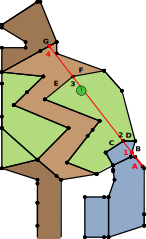
\includegraphics[width=.45\textwidth]{drawings/E1M1_slimetrail_split2.pdf}
\end{wrapfigure}
Let's position the player along the same split line we just studied but facing the opposite direction (the scene is simpler with less walls). The player still very close to segments \cw{E} and \cw{F} (which is were the rendering error is).\\
\par
The frame starts with a blank canvas. Segment \cw{E} is rendered first into the green section (labeled \circled{1} on the opposite page). Since it is a lower texture, the screen space below is inferred to be a floor and a pink visplane \circled{2} is created. Now what should have been rendered is \cw{F1}, the left part of \cw{F} which was on the left of the split. Since the split never happened, the renderer carries on (front to back) and renders \cw{G1}, the left part of \cw{G}.\\
\par
At this point in the life of this frame, things start to get weird and the bug happens.
 

\fullimage{leak_opposite_explained.png}\\
\par
Segment \cw{G1} is renderer. Its boundaries are mathematically accurate since it was an actual split so it spread juuuuust a little bit more to the right than \cw{E} \circled{3}. Three pixels more to the right to be accurate. Since \cw{G1} had a lower texture, everything in screenspace below \cw{G1} is a yellow visplane \circled{4}.\\
 \par
 After that, line \cw{F} is rendered but since the visplane already squeezed itself next to \cw{E}, it is clipped.\\
 \par
 \fixme{The description on this double page sucks. REDO IT!}
 
